\section{Metodología}

Durante la historia del desarrollo de software han surgido muchas metodologías de desarrollo ágil buscando facilitar este y asegurar su cumplimiento. Una de las metodologías de desarrollo más utilizadas es SCRUM. SCRUM fue presentado por primera vez en el artículo ``The new new Product development game'' \cite{takeuchi1986new}. Aunque inicialmente SCRUM está pensado para grupos de trabajo, en este caso será útil de aplicar ciertas partes de la metodología.

La metodología divide los actores en tres tipos de personas: Desarrolladores, Product Owner y Scrum Master \cite{schwaber2011scrum}. En este caso concreto, la metodología se planificó de forma que la tutora hiciese el rol de Product Owner asegurando que el producto llegue a buen término y que cumpla con los requisitos necesarios. Por otra parte, el alumno desarrollaría los roles de desarrollador y Scrum master. Aquí se busca ser capaz de hacerse cargo tanto del desarrollo, planear cada sprint, adaptar el plan a realizar para cada día de desarrollo, garantizar que la aplicación de SCRUM es la correcta, eliminar impedimentos del desarrollo entre otras funciones. 

Los sprints de desarrollo se fijaron en una duración de dos semanas cada uno, comenzando el día 1 de abril. En el primer día de cada sprint se realizaba la planificación de este, buscando las tareas a realizar en ese sprint en función del tiempo, y como se distribuye el trabajo en base a la carga de esas semana. Al ser un proyecto paralelo a otros, es decir, no se tenía un pleno tiempo de trabajo durante el sprint, estos se planificaban en base a la carga de trabajo externa de esa quincena. Cada día dedicado al proyecto, se planificaba las tareas a realizar ese mismo día. 

Cada día de finalización de los sprints, se realizaba una reunión de aproximadamente 30 minutos con la Product Owner buscando mejorar y corregir lo realizado durante el desarrollo. Estas reuniones normalmente aumentaban el trabajo a realizar para los siguientes sprints.

Aplicando esto, se llegó a un proceso iterativo donde cada iteración de desarrollo correspondía a un sprint. Previo a esto, se realizaron las reuniones con los clientes, para recabar toda la información necesaria y recoger los requisitos y objetivos según lo acordado. El flujo de trabajo quedaría finalmente como el indicado en la Figura \ref{fig:modelo_de_proceso}.

\begin{figure}[H]
    \centering
    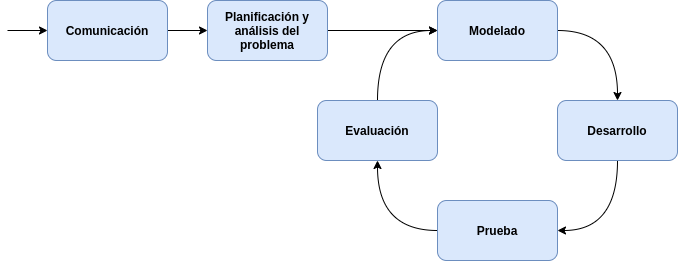
\includegraphics[width=\textwidth]{diseno/modelo_de_proceso.png}
    \caption{Modelo de proceso del proyecto}
    \label{fig:modelo_de_proceso}
\end{figure}

\section{Temporización}

Una vez decidida la metodología a aplicar, había que buscar una forma de planificar las tareas a realizar en el tiempo. Uno de los creadores de Scrum habla de como en el desarrollo de software ``generalmente el 80\% del valor de un producto de software reside en el 20\% de sus funcionalidades''\cite{sutherland-2014}. Bajo esta premisa, buscando garantizar el desarrollo de un producto completo, se ordenaron las funcionalidades en base a prioridades, garantizando de que en caso de que el producto no llegase a entregase de forma completa, se pudiese entregar una parte funcional de este.

Partiendo de lo comentado en reuniones con los clientes y de los requisitos establecidos, las partes o tareas del desarrollo se organizaron tal que así: 

\begin{itemize}
    \item Prioridad de nivel 4
    \begin{itemize}
        \item Sistemas de autenticación y de gestión de usuarios.
        \item Gestión de datos de personas sin contemplar relaciones entre ellos ni altas y bajas.
        \item Gestión de documentos asociados a las personas
        \item Gestión de datos de casas y habitaciones junto con sus residentes.
        \item Gestión de actividades y asistentes a estas sin puntuaciones.
    \end{itemize}
    \item Prioridad de nivel 3
    \begin{itemize}
        \item Uso de fotografías en personas, actividades y alojamientos.
        \item Gestión de altas y bajas de los residentes.
        \item Puntuaciones en los asistentes a las actividades.
        \item Gestión de citas asociadas a personas.
    \end{itemize}
    \item Prioridad de nivel 2
    \begin{itemize}
        \item Ranking de usuarios.
        \item Estadísticas.
        \item Búsqueda de personas por parámetros.
        \item Exportación de datos.
    \end{itemize}
    \item Prioridad de nivel 1
    \begin{itemize}
        \item Módulo de cámara insertado en la aplicación.
        \item Notificaciones de citas. 
    \end{itemize}
\end{itemize}

Estas características, algunas con más trabajo que otras, han sido ordenadas de forma que si se desarrollan las características siguiendo la prioridad establecida se podrá asegurar la entrega final de un producto válido.

\section{Seguimiento del desarrollo}
